\section{Materials}
\addtocontents{toc}{\protect\setcounter{tocdepth}{2}}
The following section presents the technical documentation of the data preprocessing, classifier implementation, and explanation generation.\newline
As described in section \ref{subsubsec:method_classifier}, we train three classifiers on a dataset of social media texts containing offensive language. The goal is to produce classifiers with varying accuracies on a testset


\subsection{Dataset}

\subsubsection{Dataset Construction}
The original dataset was collected by Davidson et al. \cite{davidson2017automated} for their research on defining and differentiating hate speech from offensive language. They constructed a dataset with offensive Tweets and hate speech by conducting a keyword search on Twitter, using keywords registered in the hatebase dictionary\footnote{https://www.hatebase.org}. The timelines of Twitter users identified with the keyword search were scraped, resulting in a dataset of over 8 million Tweets. They selected 25 000 Tweets at random and had at least 3 annotators from Figure Eight\footnote{https://www.figure-eight.com} (formerly Crowd Flower) who labelled each Tweet as containing hate speech, offensive language, or neither. They reached an inter-annotator agreement of 0.92 \cite{davidson2017automated}. The dataset is publicly available on GitHub\footnote{https://github.com/t-davidson/hate-speech-and-offensive-language}.\newline
The biggest class in the dataset are the offensive language Tweets (77\%), while non-offensive Tweets represent 17\%, and hate speech 6\% of the dataset. \newline
For our research, we are interested in offensive and not offensive Tweets. The Tweets labelled as hate speech in this dataset have characteristics that offensive language does not necessarily have, i.e. is always pejorative, while offensive language can also be found in positive contexts (see \cite{davidson2017automated}). We therefore excluded Tweets labelled as hate speech for the further construction of our dataset. We produced a balanced dataset by selecting only Tweets with the maximum inter-annotator agreement from each of the two remaining classes, and randomly drew Tweets from the bigger class (offensive Tweets) until the size of the subset was equal to the size of the smaller class (non-offensive Tweets). Table \ref{tab:StatsDataset} presents statistical information about the resulting dataset.
%-------------------------------------------------------
\begin{table}[!ht]
	\centering
	\begin{tabular}{lll}
		\hline
		\textbf{} & \textbf{Not Offensive Class} & \textbf{Offensive Class} \\ \hline
		Size (absolute) & 4,162 & 4,162 \\
		Size (relative) & 50.00\% & 50.00\% \\
		Total words & 58,288 & 61,504 \\
		Unique words & 6,437 & 9,855 \\
		\begin{tabular}[c]{@{}l@{}}Average words\\per Tweet\end{tabular} & 14.00 & 14.78 \\ \hline         
	\end{tabular}
	\caption{Statistical characteristics of the constructed dataset}
	\label{tab:StatsDataset}
\end{table}
%-------------------------------------------------------
The dataset is split into a training set and a test set, with the test set containing 20\% of the data points. The training set is used to build the classifier models, while the Tweets of the test set are used to evaluate the classifiers and to generate the data points for the user study.



\subsubsection{Dataset Preprocessing}
To prepare the data to be used in a machine learning application, we adopt the following preprocessing steps (see section \ref{subsubsec:tweet_cleaning}) in chronological order:
\begin{enumerate}
	\item Conversion of all texts to lower cases
	\item Replacement of URLs by a dummy URL (``URL")
	\item Replacement of referenced user names and handles by a dummy handle (``USERNAME")
	\item This dataset encodes emojis in unicode decimal codes, e.g. ``\&\#128512;" for a grinning face. In order to keep the information contained in emojis, each emoji is replaced by its textual description (upper cased and without whitespaces to ensure unity for tokenizing)\footnote{https://www.quackit.com/character\_sets/emoji/}.
	\item Resolving contractions such as ``we're" or ``don't" by replacing contractions with their long version\footnote{https://en.wikipedia.org/wiki/Wikipedia:List\_of\_English\_contractions}.
	\item This dataset uses a few signifiers such as ``english translation" to mark a Tweet that has been translated to English, or ``rt" to mark a Retweet (i.e. a response to a previous Tweet). Since those information have been added retrospectively, we discard them here and delete the signifiers from the texts.
	\item Replacement of all characters that are non-alphabetic and not a hashtag by a whitespace
	\item Replacement of more than one subsequent whitespace by a single whitespace
	\item Tokenization on whitespaces
\end{enumerate}
After training the classifiers, the URL and username tokens are replaced by a more readable version (``http://website.com/website" and ``@username", respectively) to make it easier for participants of the user study to envision themselves in the scenario of a social media administrator reading real-world Tweets. Replacing the tokens by their original URLs and usernames would give the participants more information than the classifiers had; we therefore chose to use a dummy URL and username.\medskip\newline

Following the preprocessing steps, the following Tweet is processed from its original form:
\medskip \hrule \medskip
\begin{verbatim}
	"@WBUR: A smuggler explains how he helped fighters along the \end{verbatim}\begin{verbatim}"Jihadi Highway": http://t.co/UX4anxeAwd"
\end{verbatim}
\medskip \hrule \medskip
into a cleaned version:
\medskip \hrule \medskip
\begin{verbatim}
@username a smuggler explains how he helped fighters along the \end{verbatim}\begin{verbatim}jihadi highway http://website.com/website
\end{verbatim}
\medskip \hrule \medskip





\subsection{Classifier}
Intro

\paragraph{Good System}
L2X, accuracy on testset

\paragraph{Medium System}
Logistic Regression with binary (1 / -1) coefficients to bring down accuracy towards the needed 0.7. In a way, \cite{klenner2018offensive} does the same, but identify the ``sign" (offensiveness) of words not by using a logistic regression classifier. In the end, it leads to the same result: with binary coefficients, the label corresponds to the class that has the most words in the sentence.
accuracy on testset

\paragraph{Bad System}
Inverse L2X
accuracy on test set



\subsection{Explanations}
reference to section \ref{subsubsec:explanation_systems}: explanations for text via highlighting of important features (here: words). 

\paragraph{Good System}
L2X mutual information

\paragraph{Medium System}
randomly choosing k words from the words with positive (offensive) or negative (not offensive) class. With logreg, a sentence of n words, all n could have the same sign (i.e. adding towards the same class). But since we use the binarised version of the coefficients (to bring down accuracy), we are confronted with n selected words. We need to choose k words to be consistent with the explanations of the L2X classifier. We therefore randomly draw k words from the set of words with the same sign.

\paragraph{Bad System}
Inverse good system



\subsection{Graphical User Interface}
\begin{itemize}
	\item the ``environment": administration tool
	\item visualisation of the decisions
	\item visualisation of the explanations (why changing text colour, why those two colours, why not gradient)
\end{itemize}

\begin{figure} [H]
	\centering
	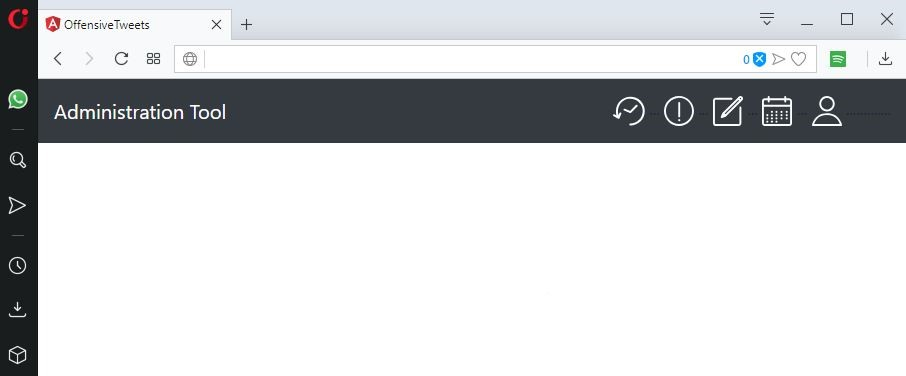
\includegraphics[width=0.8\textwidth]{img/administrationTool.JPG}\\
	\caption{Screenshot of the ``Administration Tool" to support the scenario of a social media administrator}
	\label{fig:admin_tool}
\end{figure}
\begin{figure} [H]
	\centering
	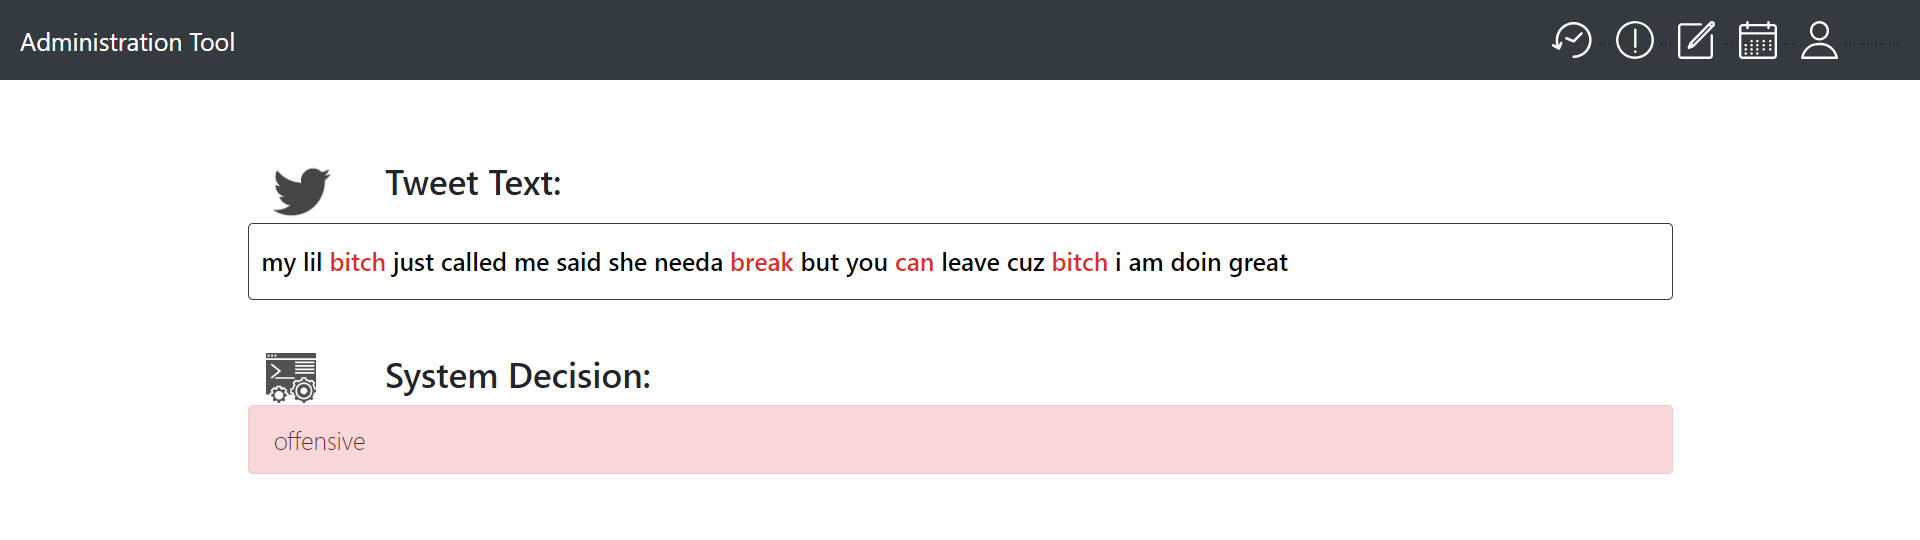
\includegraphics[width=0.8\textwidth]{img/pg_2_12.PNG}\\
	\caption{Screenshot of the ``Administration Tool" showing an offensive Tweet with explanation for its decision}
	\label{fig:admin_tool_offensive}
\end{figure}
\begin{figure} [H]
	\centering
	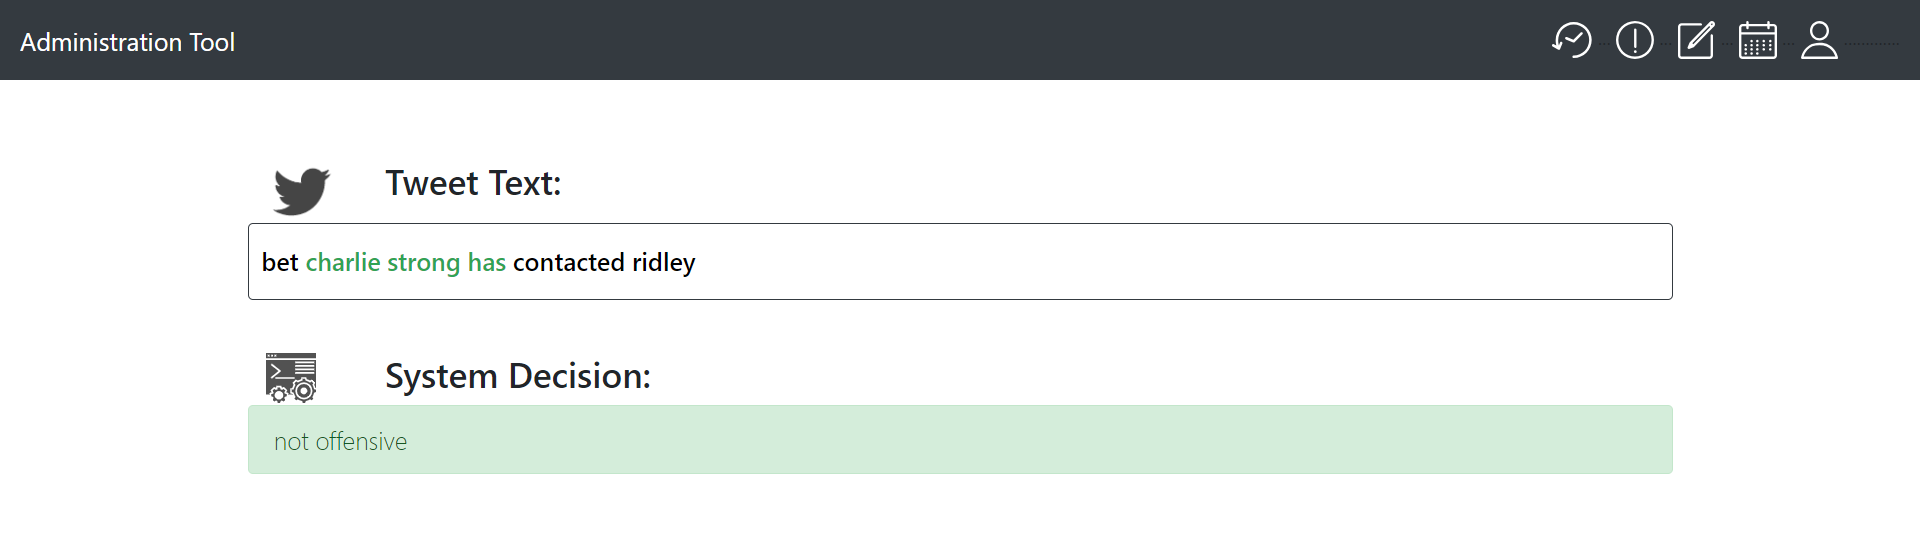
\includegraphics[width=0.8\textwidth]{img/pg_2_0.PNG}\\
	\caption{Screenshot of the ``Administration Tool" showing a non-offensive Tweet with explanation for its decision}
	\label{fig:admin_tool_not_offensive}
\end{figure}



\subsection{Subset Sampling}
For evaluating the different system-explanation conditions, users have to experience the system. However, it is not feasible to present them with the complete testeset, since it has a size of 1665 Tweets. Consequently, a subset of Tweets needs to be drawn from the testset, with a size that a human observer can understand and process within the time frame of a user study.\newline
We furthermore aim to find 10 suitable subsets and assign participants randomly to one of the subsets, in order to reduce possible side effects from biases specific to single Tweets.\newline
There are several requirements for the subsamples, originating from the conflict of reducing the sample for a human observer, yet still yielding a good representation of the testset and classifier:\newline
\begin{itemize}
	\item A class balance of the true labels similar to the testset, 
	\item a balance of correctly to incorrectly classified data points similar to the classifier's performance on the complete testset, 
	\item no overlap of Tweets within the set of 10 subsets,
	\item a feature distribution as close to the feature distribution in the complete testset.
\end{itemize}
We set the subsample size to 15 Tweets, which is enough to show accuracies to the first decimal place, yet assumably not too much to process for an observer in a user study.\newline
To create a subset, 15 data points are randomly drawn from the testset. \newline
First, the class balance of the subset is calculated. The difference to the class balance of the whole testset needs to be smaller than 0.1.\newline
Additionally, for each classifier in the user study, the prediction accuracy on the subset is compared to the prediction accuracy on the complete testset. If, for all classifiers, the difference is smaller than 0.1, the next check is performed.\newline
To ensure the uniqueness of the subsets, the randomly drawn Tweets are compared with the content of previously found subsets. The subset is only accepted if none of the contained Tweets appear in any previously found subset.\newline
In the last step, the feature distribution of the subset is tested against the features of the complete testset using the \textit{Kullback-Leibler Divergence} (KLD) metric. As the focus is directed towards the explanations (i.e. the highlighted words within a Tweet), only the explanations are used to examine the feature distribution. First, the feature distribution of the complete testset is calculated by constructing a word vector with tuples of words and their respective word counts. The word counts are divided by the total amount of words in the set, such that the sum of regularised counts equals 1. Next, a copy of the word vector is used to count and regularise the word frequencies in the subset. The result are two comparable vectors, yet the vector of the subset is very likely to contain zero counts for words that appear in the complete set but were never selected as explanation in the subset. Since the KLD uses the logarithm, it is undefined for zero counts. We use Laplace smoothing with k=1 to handle zero counts. For each classifier, the KLD is calculated and summed to a total divergence score for the subset.\newline
We generate a quantity of 100 such subsets and order them by their KLD sum. The 10 subsets with the smallest score are chosen as the final set of subsets.\newline




\subsection{Explanation Evaluation}
\label{subsec:expleval}
experiments to validate whether the explanations we generate are actually ``good" explanations and those generated with the random method are actually ``bad" explanations.


\subsubsection{Evaluation 1: Accuracy on Reduced Texts}
For each system, take generated explanations of Tweets in the test set, reduce the text to the selected words, and feed the ``reduced Tweets" into the system. Hypothesis: If the words are very informative for the classifier, the accuracy would not change. The new accuracy should then be close to the old accuracy.\newline
\begin{figure}[H]
	\centering
	\begin{subfigure}[b]{0.4\textwidth}
		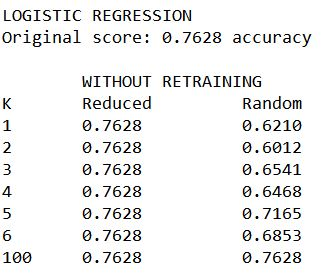
\includegraphics[width=\textwidth]{img/expleval1_logreg.JPG}
	\end{subfigure}
	\begin{subfigure}[b]{0.4\textwidth}
		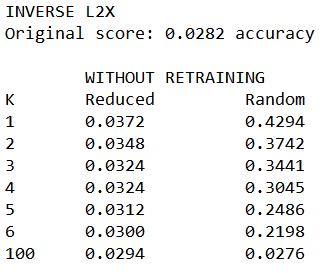
\includegraphics[width=\textwidth]{img/expleval1_invL2X.JPG}
	\end{subfigure}
	\caption{Results for evaluation of explanation experiment 1}
	\label{fig:results_expleval1}
\end{figure}
Problem: Tweets are very short, which is why the information density is high. Even when using only a single word randomly drawn from the text, the accuracy is 0.64, which is close to the medium classifier. It is therefore difficult to interpret the results for the medium classifier (0.76). Furthermore, we do not know if the Tweets have classified the same, or if only the accuracy is the same, but the mistakes were made on different Tweets. We therefore need to evaluate the ability to reproduce the very same classifications (evaluation 2).


\subsubsection{Evaluation 2: Ability to Reproduce Classifications}
For each system, divide the dataset in 5 chunks. Use each chunk once as testset and the remaining chunks as training set. This way, we get predictions and generated explanations for each data point in the dataset. Use the reduced version of the dataset with the predictions as truths to repeat the procedure of evaluation 1. Hypothesis: If the selected words are very informative for the classifier's prediction, the very same predictions can be reproduced with the reduced dataset. Since we take the predictions of the classifier on the non-reduced dataset as ``truth", the accuracy should be close to 1.0 .
\begin{figure}[H]
	\centering
	\begin{subfigure}[b]{0.4\textwidth}
		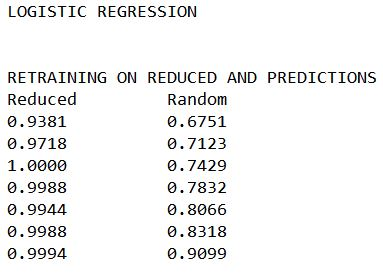
\includegraphics[width=\textwidth]{img/expleval2_logreg.JPG}
	\end{subfigure}
	\begin{subfigure}[b]{0.4\textwidth}
		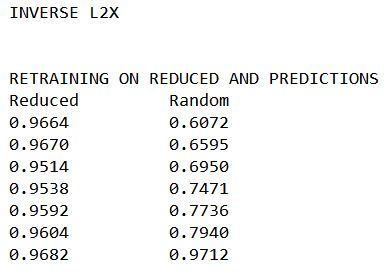
\includegraphics[width=\textwidth]{img/expleval2_invL2X.JPG}
	\end{subfigure}
	\caption{Results for evaluation of explanation experiment 2}
	\label{fig:results_expleval2}
\end{figure}



\subsection{Subset Evaluation}
same as previous section, but with the filtered subsets, basically. And on ``perfect" classifier. For k=4, because we use k=4 for final explanation generation.



\addtocontents{toc}{\protect\setcounter{tocdepth}{3}}